\documentclass[12pt]{article}
\usepackage{listings}
\usepackage{color}
\usepackage{float}
\usepackage{graphicx}

\definecolor{mygreen}{rgb}{0,0.6,0}
\definecolor{mygray}{rgb}{0.5,0.5,0.5}
\definecolor{mymauve}{rgb}{0.58,0,0.82}

\lstset{ %
	xleftmargin=2em,
	backgroundcolor=\color{white},   % choose the background color; you must add \usepackage{color} or \usepackage{xcolor}
	basicstyle=\small,%\footnotesize,        % the size of the fonts that are used for the code
	breakatwhitespace=false,         % sets if automatic breaks should only happen at whitespace
	breaklines=false,                 % sets automatic line breaking
	captionpos=b,                    % sets the caption-position to bottom
	commentstyle=\color{mygreen},    % comment style
	deletekeywords={...},            % if you want to delete keywords from the given language
	escapeinside={\%*}{*)},          % if you want to add LaTeX within your code
	extendedchars=true,              % lets you use non-ASCII characters; for 8-bits encodings only, does not work with UTF-8
	%	frame=single,                    % adds a frame around the code
	keepspaces=true,                 % keeps spaces in text, useful for keeping indentation of code (possibly needs columns=flexible)
	keywordstyle=\color{blue},       % keyword style
	language=VHDL, % the language of the code
	morekeywords={*,...},            % if you want to add more keywords to the set
	numbers=left,                    % where to put the line-numbers; possible values are (none, left, right)
	numbersep=5pt,                   % how far the line-numbers are from the code
	numberstyle=\small\color{mygray}, % the style that is used for the line-numbers
	rulecolor=\color{black},         % if not set, the frame-color may be changed on line-breaks within not-black text (e.g. comments (green here))
	showspaces=false,                % show spaces everywhere adding particular underscores; it overrides 'showstringspaces'
	showstringspaces=false,          % underline spaces within strings only
	showtabs=false,                  % show tabs within strings adding particular underscores
	stepnumber=1,                    % step between two line-numbers. If it's 1, each line will be numbered
	stringstyle=\color{mymauve},     % string literal style
	tabsize=2                  % sets default tabsize to 2 spac                  % show the filename of files included with \lstinputlisting; also try caption instead of title
}
%opening
\title{Project 2: Designing an 8-bit ALU}
\author{Adam Sumner - A20283081 \\ Contribution - 100\% \\ ~\\ ECE 485}
\date{November 16\textsuperscript{th}, 2015}

\begin{document}

\maketitle

\section{Introduction}
The purpose of this project is to implement an 8-bit ALU in the VHDL hardware-description language. The ALU should be able to perform the following functions:
\begin{itemize}
	\item ADD
	\item SUBTRACT
	\item LESS-THAN
	\item AND
	\item NOT
	\item XOR
	\item Bit Shift Left
	\item Arithmetic Bit Shift Right
\end{itemize}
\section{Design}
\subsection{Architecture}
The architecture of the ALU is simple. First and foremost, a \texttt{clk} signal is included. This is necessary because during the design process, it was concluded that all operations will be performed and outputted on the positive edge of the \texttt{clk}. Also, as per the design specification, two inputs \texttt{a} and \texttt{b} must be included. These are both signed vectors of 8 bits because this ALU is designed for 8 bit operations. They are signed because operations like addition and subtraction are included in the ALU's capability. Because in the real world negative numbers are often part of computer programs, it was necessary to make sure that the functionality of the ALU would be able to handle them. Due to the fact that signed numbers are being used, two status bits are included. These are \texttt{ov} and \texttt{zero}. \texttt{ov} is the overflow bit that is set when an overflow/underflow occurs, and \texttt{zero} is the zero status bit that is set when the output is zero. \texttt{op} is the operation bit. This signal is used to select the operation of the ALU to be performed on inputs \texttt{a} and \texttt{b}. \texttt{s} is a selector bit. Because bit shift left and arithmetic bit shift right are included in the functionality of the ALU and the ALU always takes two inputs, this signal is included to select which input to perform the shift operation on. Last an output must be included in the design of the ALU, and this is done by implementing an output \texttt{y} of 8 bits. A visual overview of the ALU is shown in Figure \ref{fig:high-level-overview}.

\begin{figure}[H]
\centering
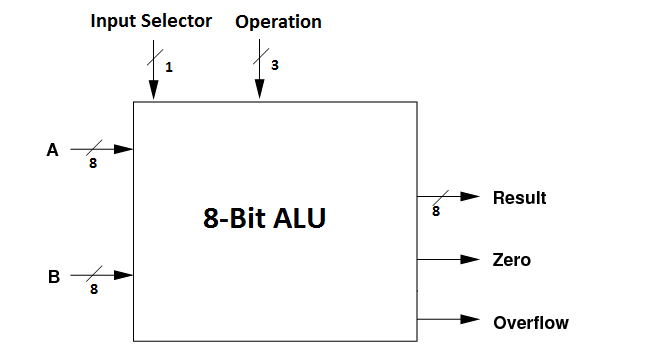
\includegraphics[width=0.7\linewidth]{high-level-overview}
\caption{High Level Overview of Architecture}
\label{fig:high-level-overview}
\end{figure}

\subsection{Behavior}
The behavior section of the code in Section \ref{sec:code} is at its core a switch case on the operation to be performed. Two bit vectors are first declared, \texttt{temp9} and \texttt{temp}. \texttt{temp9} is used in the calculation for overflow and underflow and \texttt{temp} is a temporary storage location of the result so that before its value is outputted from the ALU, its value can be checked for zero to see if the zero status bit should be set or not. A process is defined for the \texttt{clk} signal. If the \texttt{clk} is at its rising edge, then an operation can be performed. The value of the operation to be performed is then assessed. 

\begin{table}[H]
	\begin{tabular}
		
	\end{tabular}
\end{table}

\subsection{Code}\label{sec:code}
\lstset{language=VHDL}
\lstinputlisting{../alu.vhd}
\begin{lstlisting}

\end{lstlisting}

\section{Analysis}

\section{Simulation Results}



\section{Conclusion}

\end{document}
